\chapter{Example Network}
\label{system_description}

\subsection{Simulation in EPANET}
\label{example1_EPANET}

In EPANET, the simulation is built up in the same way as the network model. The simulation model is shown in the figure below. 

%EPANET example1 network
\begin{figure}[H]
\centering
\includegraphics[width=0.6\textwidth]{report/pictures/example1_epanetmodel}
% \usetikzlibrary{arrows}
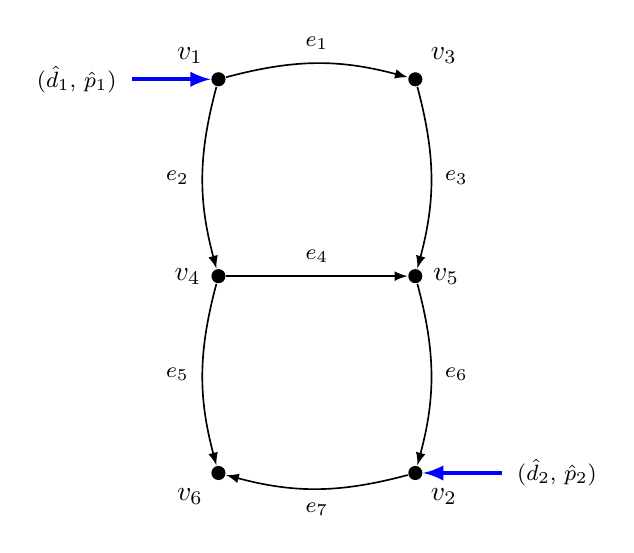
\begin{tikzpicture}[-latex ,auto,semithick,state/.style ={ draw,shape=circle,scale=1}]

\node[circle,fill,inner sep=1.8pt,label=above left: $v_1$] (A) at (0,0) {};
\node[circle,fill,inner sep=1.8pt,label=above right: $v_3$] (B) at (2.5,0) {};
\node[circle,fill,inner sep=1.8pt,label= left: $v_4$] (C) at (0,-2.5) {};
\node[circle,fill,inner sep=1.8pt,label= right: $v_5$] (D) at (2.5,-2.5) {};
\node[circle,fill,inner sep=1.8pt,label= below right: $v_2$] (E) at (2.5,-5) {};
\node[circle,fill,inner sep=1.8pt,label= below left: $v_6$] (F) at (0,-5) {};


\path (A) edge [bend right = -15] node[above  =0.05 cm] {\footnotesize$e_{1}$} (B);
\path (A) edge [bend right = 15] node[left  =0.05 cm] {\footnotesize$e_{2}$} (C);
\path (B) edge [bend right = -15] node[right  =0.05 cm] {\footnotesize$e_{3}$} (D);
\path (C) edge [bend right = 0] node[above  =0.05 cm] {\footnotesize$e_{4}$} (D);
\path (C) edge [bend right = 15] node[left  =0.05 cm] {\footnotesize$e_{5}$} (F);
\path (D) edge [bend right = -15] node[right  =0.05 cm] {\footnotesize$e_{6}$} (E);
\path (E) edge [bend right = -15] node[below  =0.05 cm] {\footnotesize$e_{7}$} (F);

\draw [-latex,line width=1.5pt,blue](-1.1,0) -- (-0.1,0);
\draw [-latex,line width=1.5pt,blue](3.6,-5) -- (2.6,-5);
\node at (-1.8,0) {\footnotesize $(\hat{d}_1$, $\hat{p}_1)$};
\node at (4.3,-5) {\footnotesize $(\hat{d}_2$, $\hat{p}_2)$};
\end{tikzpicture}
 
\caption{Non-inlet pressures in .}
\label{fig:epanet_example1}
\end{figure}

As can be seen in \figref{fig:epanet_example1}, reservoirs and pumps are present as extra links and nodes in this simulation. These extra nodes and links are removed when data is extracted from the EPANET model due to the reason that the input pressures can be measured on $v_1$ and $v_2$. The input flows can be measured through the links, connecting the reservoirs to the nodes, $v_1$ and $v_2$. Furthermore, the elevations and the demands are attributes of the nodes. In this simulation only demands are changing according to hourly time steps. 

%








